%
% PROJECT: <ETD> Electronic Thesis
%   TITLE: Looks Good to Me (LGTM): Authentication for Augmented Reality
%  AUTHOR: Ethan Gaebel
% SAVE AS: thesis-draft.tex
% 

\documentclass[12pt]{report}
%\documentclass[12pt,dvips]{report} -- ORIGINAL


\usepackage{graphicx}

\setlength{\textwidth}{6.5in}
\setlength{\textheight}{8.5in}
\setlength{\evensidemargin}{0in}
\setlength{\oddsidemargin}{0in}
\setlength{\topmargin}{0in}

\setlength{\parindent}{0pt}
\setlength{\parskip}{0.1in}

% Uncomment for double-spaced document.
% \renewcommand{\baselinestretch}{2}

% \usepackage{epsf}

\begin{document}

\thispagestyle{empty}
\pagenumbering{roman}
\begin{center}

% TITLE
{\Large 
Looks Good to Me (LGTM): 
Authentication for Augmented Reality Using Wireless Localization and Facial Recognition
}

\vfill

Ethan D. Gaebel

\vfill

Thesis submitted to the Faculty of the \\
Virginia Polytechnic Institute and State University \\
in partial fulfillment of the requirements for the degree of

\vfill

Master of Science \\
in \\
Computer Science and Applications

\vfill

Wenjing Lou, Committee Chair \\
Ing-Ray Chen \\
Guoqiang Yu 

\vfill

May 15, 2016 \\
Falls Church, Virginia

\vfill

Keywords: 
\\
Copyright 2016, Ethan D. Gaebel

\end{center}

\pagebreak

\thispagestyle{empty}
\begin{center}

{\large Looks Good to Me (LGTM): 
Authentication for Augmented Reality Using Wireless Localization and Facial Recognition}

\vfill

Ethan D. Gaebel

\vfill

(ABSTRACT)

Augmented reality is a powerful new computer interface paradigm that is going to reshape how people interact with computers. The diverse hardware on typical augmented reality headsets presents an opportunity to the security community to re-make how authentication is carried out, making it more usable for the everyday user and moving authentication away from the cloud and back to face-tof-face interactions (when users are face to face anyway). In this paper we explore an authentication protocol to be used when users are face to face and have augmented reality headsets. This protocol uses the same idea behind how humans identify speakers: localizing a wave and comparing its location to a face's location, except here we deal with radio waves instead of sound waves. This protocol is designed to minimize the work required by the user, thus increasing the likelihood that it will be used and decreasing the likelihood of user error. We provide an implementation of the protocol as well.

\vfill

\end{center}

Security-based abstract and stuff!!!

\vfill

% GRANT INFORMATION
This work was supported in part by the National Science Foundation under Grants 
CNS-1443889, CNS-1405747, CNS-1446478, and CNS-1343222.

\pagebreak

% Dedication and Acknowledgments are both optional
% \chapter*{Dedication}
% \chapter*{Acknowledgments}

\tableofcontents
\pagebreak

\listoffigures
\pagebreak

\listoftables
\pagebreak

\pagenumbering{arabic}
\pagestyle{myheadings}

%%%%%%%%%%%%%%%%%
\chapter{Introduction}
\markright{Ethan D. Gaebel \hfill Chapter 1. Introduction \hfill}
% Augmented Reality
% ---- Convince readers it is the future
% ---- Discuss options for AR: headsets, hardware included, etc
% ---- Augmented reality NEEDS a device pairing mechanism
% ---- Why pair point-to-point?
% -------- More efficient network resource usage
% --------- Problem is inherently local
% -------- Not reliant on infrastructure, more robust to patchy areas
% ------------ Cheaper if we consider the non-WiFi usage 
% ---------------- WAY cheaper if you further consider the content size!
% ---- Preserves privacy
% Augmented reality needs device pairing
% ---- Sharing holograms, etc
% Device Pairing
% ---- Difficulty of bootstrapping authentication
% ---- Man-in-the-middle (MOVE)
% ---- Evil twin (MOVE)
% ---- The Resurrecting Duckling (MOVE)
% ---- Long history, briefly summarize to illustrate the breadth of techniques investigated
% ---- Difficulty of pairing over wireless channel 
% ---- Usability's importance to security in practice
% ---- Pin currently dominant method
% ---- Mention centralized device pairing methods.... (this is kind of out of the purview of device pairing; a user account can be used to bootstrap?)
% Augmented reality can have BETTER device pairing
% ---- Improved hardware and user interface provides avenue for BETTER device pairing (better = more usable --> more secure)
% -------- Must be more usable than a pin
% High level description of LGTM from the user perspective (high level even for the user view)
% ---- Press button, look at other person, etc
% ---- Compare EM waves & sound waves for localization & information carrying purposes
% ---- How does this look formally? (transition)
Augmented reality is one of the most exciting new technologies on the horizon, promising three-dimensional interfaces that one or more users can directly interact with. Augmented reality is most commonly provided via a head-mounted display with translucent lenses having digital content in two or three dimensions rendered on top of the real world. Many of these head-mounted displays will be full stand-alone computers equipped with powerful processors, wireless communications, one or more high resolution cameras, and depth sensors. Stand-alone head-mounted displays require much of this sophisticated technology to provide fully interactive augmented reality which, at a minimum, requires hand tracking, graphics processing, and wireless communication, since connectivity is a requirement for any consumer device today. 

Users of augmented reality headsets have the same need that users of any other consumer electronic device have today: the need to send content to others. In the case of augmented reality, this content will often be far richer, and thus larger, than we've seen on other platforms, since users will be creating, viewing, and working with three-dimensional objects, which inherently have more information associated with them than their equivalent two-dimensional representations. It is also likely that users will want to share content face to face, providing 3D objects that both users can see and/or interact with in real time; most smart phone users have looked up a video or picture to show someone. In fact, we can expect this type of sharing to increase with augmented reality so that users are sharing app interfaces, sharing group photos in real-time, and passing secret three-dimensional jokes back and forth constantly, just like they send snaps on Snapchat today.

Content sharing between users in close proximity is an interesting and well-studied $[CITATIONS]$ problem. Typical content sharing schemes today take advantage of pre-existing infrastructure via cell towers, wireless access points, and the Internet. This makes very good sense considering the most common use case for digitally sharing content is to share it with those who aren't present; you wouldn't send someone standing next to you a video. But with augmented reality you would send someone sitting next to you a video so that the two of you can watch it together through your respective headsets. Since this type of sharing will be so pronounced, it deserves separate consideration from the general content sharing problem, which is why point-to-point wireless communication should be used for such content sharing, particularly when the content is stored locally on a user's device, as would be the case with photographs, three-dimensional scene captures, videos, and user-created three-dimensional content. By sharing content directly from person-to-person network resources are saved, money may be saved if charge-by-data-usage plans are being used for Internet access. Person-to-person content sharing is robust in the face of local or global infrastructure failures, and content sharing privacy details, such as who is communicating with whom, what is being communicated, and when the communication is occurring, are kept between the two users doing the sharing instead of being shared with whatever entity (or entities) is (are) providing the service. 

There are many options for point-to-point wireless communication but a full discussion and evaluation of these options is outside the purview of this thesis. However it is relevant to briefly mention some major enabling technologies so as to convince the reader of the feasibility of such a design, so I will briefly mention a few common technologies. WiFi Direct $[CITATION]$ is perhaps the simplest since any WiFi-capable device can take advantage of it with the right software. WiFi Direct also has direct support via the application programming interface (API) in the popular Android operating system. Bluetooth also includes a point-to-point protocol, with support in Android, iOS, and most modern computers. 

% Begin exposition on my problem
When working in a point-to-point wireless communications scenario, authentication can be tricky. It will often be the case that two users have not used their devices to communicate before, so there will be no pre-existing security context (such as a pin, key, token, etc.) between the two devices. 

Device pairing is the area dedicated to authenticating devices without prior security context, and there have been many schemes introduced to address this problem on devices with myriad hardware features and constraints. To give a quick idea of the breadth of the techniques proposed, some schemes have involved: screens with changing bar codes, infrared communication, blinking lights, communicating cryptographic keys using speakers and microphones, and numerical pin entry. All of these methods rely on communication over one or more out-of-band channels, which is a channel using human sensory capabilities to authenticate other communication channels that are imperceptible to humans, which is usually the wireless channel. To authenticate the human imperceptible channel, some key is transmitted over the out-of-band channel which is then used for authentication. The simplest, and most common, example is that of a numerical pin. A pin may be permanently bound to a device without a user interface, and the user enters the pin into another device with a user interface to perform authentication; this is the case with Bluetooth headsets.

These out-of-band channels explicitly require a human to participate, and it may be expected that the human actor has some impact on the security of the scheme as a result. This intuition has been validated in $[CITATIONS]$ where comparative user studies were conducted between several different device pairing techniques. In $[CITATION--Usability Analysis of Secure Device Pairing Methods]$ two rounds of usability tests were performed for two different methods: compare-and-confirm and select-and-confirm. For these methods, users had to compare a randomly generated pin presented on each device for equality and confirm if they matched, and select a pin from a list on one device sent to it from the first device and confirm if they matched, respectively. Each method was measured by fatal error rate and total user error rate, where a fatal error is an error that results in a security breach and total user error is all the fatal errors combined with all errors that do not result in a security breach (only user annoyance). The two rounds of usability tests differed in the user interface the study participants used, while also being performed on different users. In the first round, compare-and-confirm had a fatal error rate of $20\%$, and select-and-confirm had a fatal error rate of $12.5\%$, while compare-and-confirm had a $20\%$ total error rate, and select-and-confirm had a $20\%$ total error rate. The researchers suspected that the user interface could be the problem and so improved the interfaces, as well as lengthening the pins from 4 numbers to 6 numbers, the idea being that a longer pin will force users to focus more on the task, making them less likely to make a mistake. In the second round, compare-and-confirm had a fatal error rate of $0\%$, and select-and-confirm had a fatal error rate of $5\%$, while compare-and-confirm had a $2.5\%$ total error rate, and select-and-confirm had a $7.5\%$ total error rate. So we see that these results mirror our intuition regarding usability's effect on the security of device pairing schemes. Furthermore, making authentication easier for the user is a worthy goal in and of itself. A hallmark of technology in general has been making certain things easier for the masses, so it should be with security technology. 

Augmented reality presents a new computing platform with many required hardware and software features that have not been previously seen on consumer devices. These hardware features present an opportunity for a better device pairing scheme that is both more secure and more usable. Think of how two people who have never met before authenticate one another while speaking. Sound waves are localized and paired with the face we see at the point of localization. Afterwards we know the sound of the person's voice and can recognize it without seeing them. Can we do something similar with the hardware available in an augmented reality headset? Yes. We can localize the wireless signal and digitally overlay its location with a box or other type of indicator on reality for the user to view, and use facial recognition to locate a face fitting a model transmitted to our device and overlay a box around the face recognized in the current frame. The user can then verify on the digital overlay that the wireless signal is emanating from the person they would like to communicate with. If user finds that the person their device recognizes is who they want to communicate with and that the wireless signal is indeed coming from them, the user can say to themselves, ``looks good to me!'' and indicate that the other user has been authenticated. This is the basic view of how my system will work from the user's perspective, but lets move on to the next section to formalize this protocol and everything that happens under the hood.


%%%%%%%%%%%%%%%%%
\chapter{Protocol Design}
\section{System Model}
% System Model
% ---- Protocol hardware requirements
% -------- Users have augmented reality head-mounted displays equipped with:
%               wireless communications, support for point-to-point 
%               communications, high resolution cameras, relatively good 
%               computational abilities, and translucent screens very close to 
%               the eye such that only the user can reasonably see them which 
%               are capable of rendering 2D and 3D objects on top of the 
%               physical world which the user is already seeing.
% ---- Users are present, in-person/face to face, and would like to establish 
%           communication to share some kind of content between their devices 
%           which may include: a shared app experience, watching a video, 
%           listening to the same music, shared holograms, basic messaging
% ---- Users of LGTM have no prior security context with regard to their 
%           devices; the users may be friends, acquaintances or strangers.
% ---- Each user possesses, in the memory of their augmented reality headsets, 
%           facial recognition models for themselves.
% -------- These are easily trained via mirror.
% ---- No assumptions regarding access to the Internet are made.
First we must adequately understand the scenarios where the Looks Good to Me (LGTM) protocol is applicable. This requires us to go down the list of: hardware requirements, security context, the users' context, and any other assumptions made. 
LGTM is specifically designed for authenticating two users, Alice and Bob.
% however it is simple to extend this scheme to multiple users by allowing Alice and Bob to individually perform authentication while the other party participates in the final approval (but not the full protocol itself).

LGTM assumes that users are equipped with head-mounted augmented reality rigs, each of which possesses: wireless communications hardware with support for a point-to-point communication protocol, a high-definition video camera, and a translucent display directly in front of the users' eyes that is capable of displaying digital objects on top of the physical world (this last requirement is satisfied simply by the users possessing head-mounted augmented reality rigs, but we want to be thorough). 

The two hardware devices are assumed to have no prior security context, which means the two devices do not possess any information that can be used to prove the authenticity of their claimed identity to the other. A pre-shared key is a common example of a piece of information which can be used as pre-existing security context.

An important piece of information that each headset is assumed to possess is a facial recognition model capable of recognizing the user of the headset. That is, Alice's headset has a facial recognition model that can recognize her, and Bob's headset has a facial recognition model that can recognize him. Training for these models can be done easily in a mirror.

As for the users themselves, Alice and Bob are assumed to be in sight of each other and would like to share some sort of digital content with one another, such as: a shared application experience, a shared video, shared music, shared holograms, or basic messaging. No assumptions are made of Alice and Bob's relationship with each other: they may be friends, acquaintances, or strangers.

No assumption regarding access to the Internet is made. 

\section{Security Objectives}
% (Security) Objectives
% ---- Authenticate the wireless signal of one user so that secure 
%           communication can be done between two individuals
% -------- Bootstrapping authentication
% ---- Select a user-wireless signal pair to communicate with
% -------- Selection problem
% ---- Privacy Objectives (sub-section under security objectives...)
% -------- No need for centralized power knowing communication/content patterns
% -------- Intermediary parties facilitating communication is 0
% ------------ The potential for remote eavesdropping, censorship, tracking, 
%                   etc, is non-existent
The primary security objective is for Alice and Bob to correctly authenticate one another's wireless signals so that they can engage in secure point-to-point wireless communication. Recall from the system model section that Alice and Bob do not share any security context, so this authentication must be bootstrapped. 

A secondary objective is for Alice and Bob to correctly select which (user, wireless signal) pair they want to communicate with. This objective is directly related to the first but it warrants distinction as a worthy problem on its own merit since there are many practical attacks that rely upon tricking users into selecting the wrong thing $[CITATIONS, DIVERSE ONES]$. We refer to this as the selection problem.

There is a final security objective which is perhaps more accurately described as a privacy objective. That objective is for there to be a guarantee that no outside parties are aware of the communication or content patterns present for any user of LGTM. Specifically, this means that it is not possible for an outside entity, one not directly engaging with Alice, to determine who she communicates with or what she communicates. 

\section{Threat Model}
% Threat Model
% ---- Wireless attacker model
Attackers have quite a bit of power when dealing with a wireless channel since the communications medium is both public and localized. Attackers have the capability to: jam communications, perform denial-of-service attacks by flooding the channel with packets constructed to fit the protocol, eavesdrop on all packets transmitted, and replay packets collected from eavesdropping in any order. Further, the attacker may have multiple transceivers at his or her disposal, so attacks can be coordinated between more than one node.
Attackers may use these capabilities to accomplish one or several goals. An attacker may want to impersonate Alice to send Bob falsified content. An attacker may want to impersonate both Alice and Bob to perform a man-in-the-middle attack allowing them to eavesdrop on encrypted communications between Alice and Bob. The attacker may simply want to prevent communication between Alice and Bob. Or the attacker may want to do any of the above steps with the higher goal of exploiting some subsystem.

\section{Protocol}
% Protocol, high level (high-level, as in the protocol diagram)
Alice and Bob are two individuals wearing augmented reality headsets equipped with a high-definition camera, point-to-point wireless communication abilities, and computational ability equal to the average laptop computer. Alice presses a button, which may be holographic or physical, and begins listening. Bob presses a button as well which opens his headset up to listening and also sends an initialization packet to Alice with his network identification, a random nonce, a public key, and some initialization text. Alice receives this message and responds by transmitting her public key and a nonce encrypted with Bob's public key. Alice and Bob both generate a session key using $nonce_A$ and $nonce_B$ which both parties now possess. Bob encrypts facial recognition parameters and a cryptographic hash of all messages sent between Alice and Bob using the shared session key and broadcasts this. Alice receives Bob's message, decrypts Bob's facial recognition parameters verifies the included hash of all prior messages, and extracts channel state information from the wireless signal carrying the facial recognition parameters. Alice responds by encrypting facial recognition parameters to recognize herself with a cryptographic hash of all their previous messages concatenated using their shared session key. Bob receives Alice's encrypted facial recognition parameters, decrypts them, verifies the concatenated hash, and extracts channel state information from the wireless signal which carried the facial recognition parameters. Now, Alice and Bob each run localization algorithms using the channel state information as input and locate the origin of the signal sources. Then, Alice and Bob run facial recognition algorithms using the facial recognition parameters they received from each other and locate each other's faces (if they are currently in each other's field of view). It is expected that in practice Alice and Bob will receive many of these correspondences, so the protocol automatically tosses out any facial recognition-signal location pairs where the signal location is not overlapping with the face position. I say overlap, because in practice there will be an error tolerance on the signal location, so rather than a single point, there will be a sphere where the signal may have originated from. Invalid pairs of wireless signals and facial recognition parameters having been thrown out, Alice sees a square drawn around Bob's face on the augmented reality headset screen and Bob similarly sees a square drawn around Alice's face on the augmented reality headset screen. They are both prompted to accept or reject the face selected by the protocol. If they both accept, Alice and Bob begin communicating normally using a channel encrypted with their shared session key. \\

% Protocol Figure
\begin{figure}
\center
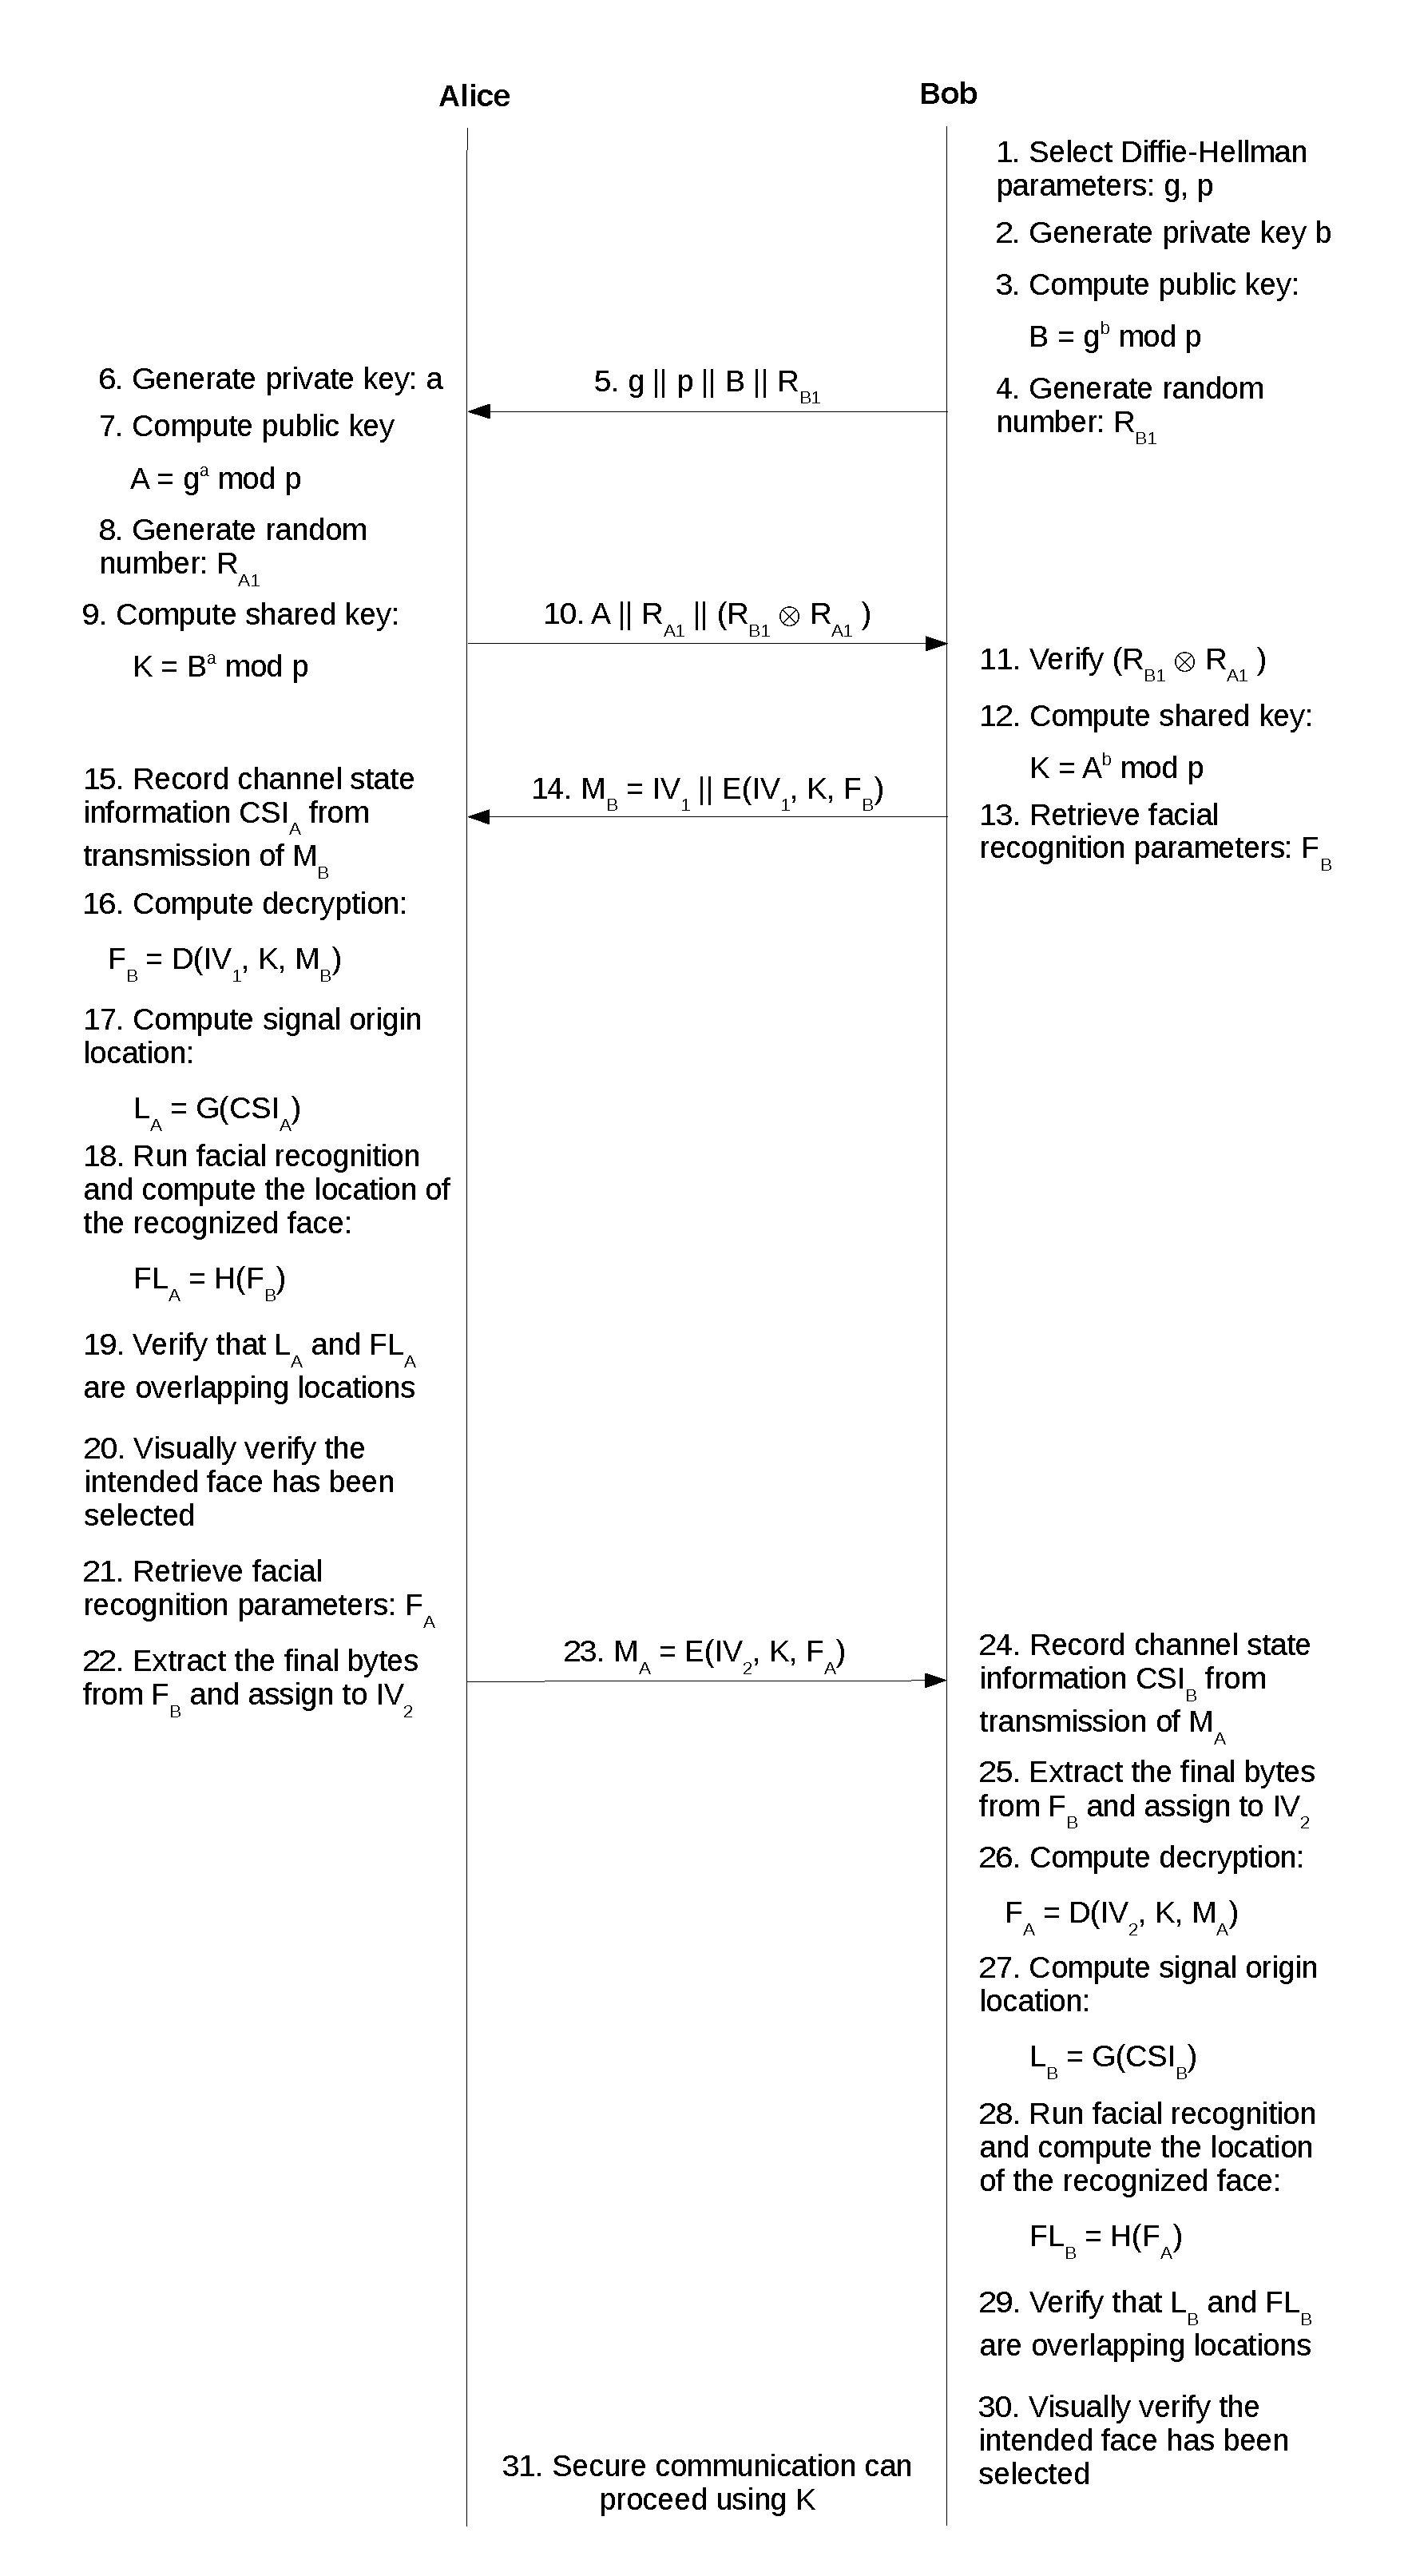
\includegraphics[scale=0.6]{../figures/looks-good-to-me-protocol-diagram.pdf}
\caption{Looks good to me protocol diagram...}
\label{protocol-diagram}
\end{figure}

% Protocol, specific (Alice receives $n$ packets, etc...)

\section{Analysis}
% Protocol Analysis
% ---- Describe each step of the protocol (protocol specific above?)
The LGTM protocol uses many different techniques to bootstrap authenticated communications between two users. Here I will go into some detail as to why each of these techniques was included. \\

Symmetric key encryption is bootstrapped from asymmetric key encryption in the first few messages. This is done in the usual way and is very similar to other protocols $[CITATIONS]$. Hash based message authentication codes are used to authenticate messages as belonging to a single user. \\

The security of LGTM mostly relies upon wireless localization. A user can successfully authenticate another user by comparing the location obtained via wireless localization and comparing it to the location of the user they're attempting to authenticate. \\

Facial recognition is used to boost usability. Humans are excellent at recognizing other humans faces. Infants as young as <LOOK UP> $[CITATION]$ have shown the ability to distinguish between different faces. Using intuition gleaned from this, I have decided to incorporate facial recognition into this scheme so that users need only look at a face and confirm it to authenticate. This is an easier task than identifying whether a particular person's head overlaps with a sphere. The usability of a security scheme, specifically pairing, has been found to directly affect the actual security of a scheme, since user error resulting from unfriendly user interfaces can result in security issues occurring.


\subsection{Security}
% Security
% ---- Wireless attacks
% -------- Jamming 
% ------------ Works on any wireless pairing technique
% -------- DOS, spam the user(s) with auth requests 
% ------------ Works on any wireless pairing technique
% -------- Man-in-the-middle
% ------------ Works on any wireless pairing technique
% ------------ Wait...the feasibility depends on the quality of the wireless 
%                   localization. In a perfect implementation, this won't work.
% ---- Attacker ability is based on the quality of the facial recognition 
%           & wireless localization (correctness)
% -------- "Attack space" for wireless localization
% ---- Why not a pin?
LGTM is robust in the face of many attacks which other device pairing schemes fall to. 

\subsubsection{User Impersonation via Imprecise Wireless Localization}
As stated above, LGTM relies heavily on wireless localization for security, and so it should come as no surprise that imprecise wireless localization can result in serious security issues for LGTM. Consider Alice and Bob are face-to-face with one-another and an attacker, Eve, is close enough to Bob so that wireless localization will confuse the two of them. Eve can obtain a valid facial recognition model for Bob either by communicating with him via LGTM or by gathering photographs of Bob and training her own model. Now that Eve has Bob's facial recognition parameters, Eve can initiate LGTM at the same time as Bob, while also sending Bob's facial recognition parameters. Alice will localize Eve's signal to be overlapping with Bob, and will also receive Bob's facial recognition parameters. So Alice will now have essentially two Bob's which she must choose from. If Alice selects Eve, then Eve is now free to impersonate Bob, until she is found out. In scenarios where silence is for some reason required, Eve may be able to pull this impersonation off for some time, perhaps long enough to exploit another system. \\

\subsubsection{Man-in-the-Middle}
Man-in-the-middle attacks plague all device pairing schemes since it is a notoriously hard problem to bootstrap trust and prevent someone from stepping in-between the two users pairing and impersonating both of them, since authenticity is not yet established. LGTM's localization helps significantly with this common problem by identifying the location of a device transmitting. So with a localization technique that works well, man-in-the-middle attacks are not possible. However, realistically localization remains a difficult problem with very recent schemes $[CITATIONS]$ being responsible for making LGTM feasible at all. These recent schemes are still not precise enough to totally remove the possibility of man-in-the-middle attacks. So it is possible for an attacker to impersonate both users, perhaps using separate but cooperating transceivers, and facilitate the authentication between both users while eavesdropping on the key exchanged. A very powerful attacker will be able to achieve this, but it will require very creative jamming. Eve will have to jam Bob enough so that Alice does not receive his messages, but Eve does and likewise with Alice. The rest of the attack proceeds with Eve merely carrying out both sides of the authentication to each opposing user, culminating in Alice and Bob having a shared key, which Eve also has and uses to eavesdrop on every communication Alice and Bob send to one-another. \\

Man-in-the-middle attacks plague all device pairing systems, but I believe it has been made better by LGTM due to the addition of localization. \\

\subsubsection{Jamming}
Jamming is a very simple attack. Eve merely broadcasts on the frequencies Alice and Bob are attempting to communicate on and overpowers and communications abilities that the two may have, rendering them unable to communicate at all over the wireless channel. This is one form of denial-of-service attack, we shall look at another one in the next step.

\subsubsection{Denial-of-Service}
Denial-of-service is often used very generally, but here it is a very specific way for Eve to ruin Alice and Bob's communication. Eve can spin up many instances of LGTM when she sees Alice and Bob initiating it and Eve can legitimately go through the protocol with Alice and Bob until the end when it is time to authenticate the user. By spamming Alice and Bob Eve wastes valuable time and ties up system resources, which are significant due to the high computational costs incurred by wireless localization and facial recognition. In this manner, Eve can endeavor to make authentication take longer than is acceptable, or if she persists, Eve may even be able to exhaust Alice or Bob's device batteries.

\subsection{Usability}
% Usability
% ---- Why not a pin?
% -------- Greater range; you can see farther than you can hear
% -------- Will not work in loud environments
% -------- Will not work for the deaf (LGTM won't work for the blind, but 
%                   neither will AR in general, and neither will a pin)
% -------- Depending on implementation, may be less secure, overhearing 
%                   pin can be a security leak
LGTM has usability at the core of its design and indeed pays a high price to maximize usability. As mentioned before, the facial recognition parameters are purely for usability purposes, and transmitting these recognition parameters is not cheap. It is my firm belief that this is worth it, because of the elegant simplicity that it affords LGTM. Usability is often judged by the number of user actions: LGTM requires two actions on the part of the user, initiation and confirmation. It is difficult to imagine a simpler protocol. \\

Many device pairing methods are used every day in protocols like Bluetooth. In the case of Bluetooth the users are prompted to confirm that the pin number appearing on both devices is the same. Intuitively this sounds usable enough, however in a usability study conducted by $[CITATION WORK]$ in $[CITATION]$ it was found that this pairing method resulted in security errors with 20\% of users; meaning that users confirmed that mis-matched pins matched, authenticating the incorrect device. User choice is a huge problem point in security in general. Phishing attacks rely solely upon user incompetence and these are some of the most successful and common attacks $[CITATON FOR PHISHING COMMENTS]$ used in the real world. \\

Beyond security concerns, not relying on a string comparison has other benefits. When two or more users are pairing devices they are usually relying on telling one-another what their displayed pins are vocally. This has a shorter range than the visual identification required in LGTM, and also might fail if the two users are in a loud place such as a concert. Further, this pin exchange will not work for deaf people. The deaf can resort to writing down their authentication strings, but I don't think any significant argument needs to be mounted to show that this is not a usability win. \\

<NOT SURE IF THIS GOES HERE> \\
An often un-mentioned aspect of usability is availability. LGTM does not rely on any infrastructure to perform authentication. No Internet connection, no central authority, no account information, etc. This property of LGTM is particularly appealing as it allows people to share content anytime, anywhere, for free. A common case that even the most privileged experience is ending up on an airplane where the WiFi is: first, behind a pay wall, second, slow, and third might not be working currently and there's nothing that can be done about it. Usability should consider the availability of the technology, and LGTM's only limitation on availability is the functionality core hardware on an augmented reality headset and a charged battery. \\

LGTM relies on a a very minimal set of user actions, which is achieved by offloading a lot of preprocessing steps to the augmented reality headsets. LGTM remains usable under various common situations where the currently most popular $[CITATION???]$ string comparison method does not suffice. I believe that LGTM is closing in on the simplest authentication scheme that is possible. \\

\subsection{Privacy}
% ---- Privacy
Users today are becoming more and more concerned about privacy. A study by $[CITATION STUFF]$ found that $<\%>$ of people have taken steps to increase their level of privacy online $[CITATION]$. By performing authentication over point-to-point wireless communications LGTM preserves privacy by keeping local content sharing details in the immediate area, as opposed to going through a central authentication authority which would likely capture sharing data and meta-data for various purposes. \\

\subsection{Potential Alterations}  % Should this section be here?
% Expanding to the group case
% One way sharing: (I.E. Alice receives content from Bob, but not vice-versa)
Ehhhh, maybe I'll actually include this in the final.... \\

%%%%%%%%%%%%%%%%%
\chapter{Implementation}
% General setup
% ---- AR headsets unavailable (expensive, not powerful enough yet, not 
%           flexible enough yet)
% ---- Necessary components from AR headsets for experimental purposes (
%           Wireless, video camera, display)
% Wireless Localization Discussion
% ---- Discuss past localization techniques, BRIEFLY
% ---- Discuss lack of focus on point-to-point localization
% ---- Discuss new protocols that enable point-to-point localization in 
%           commodity hardware
% Facial Recognition Discussion
% ---- Very brief discussion of techniques, the area is well studied and my 
%           techniques are not new
% Specific Wireless localization and facial recognition methods
% ---- SpotFi
% ---- OpenCV
% -------- Fisherfaces, LBPH, Haarcascade, etc
% Specific localization & facial recognition components
% ---- Intel 5300 firmware etc
% ---- Laptops with web cams and three antennas each
% System and Validation
% ---- Glue code, system structuring, specifics of protocol implementation
% ---- Explain each implementation decision, why and how, discuss alternatives
% ---- This section should mainly discuss why certain things were NOT done, 
%           and why things ARE done 
% -------- belongs under "General Setup"
\section{Introduction (Change this to a more appropriate title)}
Stand-alone augmented reality headsets are currently quite expensive; the Microsoft HoloLens development kit which was just released comes in at \$3000 USD. On top of the price, there is not currently, to my knowledge, any stand-alone augmented reality headset that has a wireless card allowing users to access channel state information, which is a requirement for wireless localization. Suffice to say, it is not currently possible to implement LGTM in its proper environment. However, we need only look at the required components for LGTM and construct a test rig that satisfies these requirements. The base requirements are: point-to-point wireless communication, the ability to localize the same point-to-point wireless communication, a high-definition video camera, a screen, some sort of user input, and for a face to be adjacent to the wireless signal origin point (so that the wireless signal can be properly paired with a face). These requirements can be fulfilled using a laptop, some specialized Intel wireless card firmware, an array of three antennas, a web cam, and a picture of someone's face stuck on the back of the laptop. This setup, although strange, suffices to properly implement LGTM.

\section{Hardware}
The laptops used are all Fujitsus, two of them are Fujitsu LifeBook T900s and the third is a Fujitsu LifeBook T901. The T900s are equipped with: $<INSERT HARDWARE SPECS FOR THE T900s>$. The T901 is equipped with 8 GB of RAM and a 2.5 GHz Intel i5-2520M processor with 4 cores. All three laptops had an additional second wireless card added for the experiments; the Intel 5300 AGN wireless card with three external antennas as pictured in figure $<INSERT FIGURE LABEL>$. The three external antennas were placed on the backs of the laptop with Velcro and spaced exactly 10 cm apart. The three laptops all used the same external web cam for this implementation, the Logitech C270 720p web cam, which has a 60 degree field of view. \\

\section{Software}
The software used in this implementation was quite varied, and as such it will be broken up into sections describing the implementation for each segment, followed by a description of the glue software used to make it all run together. \\

\subsection{Wireless Channel State Information Retrieval}
First and foremost, credit must be given to the researchers in $[HALPERIN CITATIOn]$ for creating custom firmware for the Intel 5300 AGN wireless card. This firmware permits recovery of channel state information from each packet received using $<GROUPINGS JARGON>$ to get 30 total readings from the subcarriers. This nets a total of 90 sensors to run signal processing code on. \\

\subsection{Point-to-Point Wireless Communication}
The firmware mentioned above also allows users to broadcast on a specified frequency with no formal connection being made. This creates a realistic adversarial wireless environment where any user can overhear any other. \\

\subsection{Wireless Localization}
Wireless localization is an old problem which has been getting more sophisticated and precise in the recent years. \\

\subsection{Facial Detection and Recognition}
Facial detection and recognition are very interesting areas of research. OpenCV, started by Intel in $<INSERT YEAR>$, is an open source computer vision library that provides easy-to-use vision APIs out of the box. In particular, I took advantage of the face detection provided by the Haarcascades technique and experimented with all three facial recognition techniques provided: Fisherfaces, Eigenfaces, and the Local Binary Pattern Histograms (LBPH) technique. \\

\subsection{Main System Software}
I took advantage of the myriad general tools provided by the Linux operating system and chose to tie together all of the above software with the Bourne-again Shell (BASH). \\


%%%%%%%%%%%%%%%%%
\chapter{Experiments}
% Experiments (Very formal)
% ---- Security
% ---- Performance
% ---- SpotFi Accuracy
% -------- Effective "attack space"
% ---- Facial recognition accuracy
% Results (for each above)
% Discussion (for each above)

%%%%%%%%%%%%%%%%%
\chapter{Conclusion}
% List of points to hit on:
% ---- Oldness and difficulty of device pairing
% ---- Usability's impact on security
% ---- Ease of use of LGTM
% ---- Point-to-point communication providing privacy
% ---- Something optimistic and feel-good sounding about the future

%%%%%%%%%%%%%%%%%
%
% Include an EPS figure with this command:
%   \epsffile{filename.eps}
%

%%%%%%%%%%%%%%%%
%
% Do tables like this:

% \begin{table}
% \caption{The Graduate School wants captions above the tables.}
% \begin{center}
%  \begin{tabular}{ccc}
%  x & 1 & 2 \\ \hline
%  1 & 1 & 2 \\
%  2 & 2 & 4 \\ \hline
%  \end{tabular}
% \end{center}
% \end{table}

%%%%%%%%%%%%%%%%%%%%%%%%%%%%%%%%

% If you are using BibTeX, uncomment the following:
% \thebibliography
%
% Otherwise, uncomment the following:
% \chapter*{Bibliography}

% \appendix

% In LaTeX, each appendix is a "chapter"
% \chapter{Program Source}


\end{document}